\documentclass[a4paper, oneside, openright]{book}

% --------------------------
% ---- DECLARE PACKAGES ----
% --------------------------
\usepackage[T1]{fontenc}
\usepackage[utf8]{inputenc}
\usepackage[english]{babel}
\usepackage{lmodern}
\usepackage[a4paper,top=2.5cm,bottom=2.5cm,left=3cm,right=3cm]{geometry}
\usepackage[fontsize=12pt]{scrextend}
\usepackage[parfill]{parskip}
\usepackage{amsmath}
\usepackage{amssymb}
\usepackage{graphicx}
\usepackage{booktabs}
\usepackage{longtable}
\usepackage{float}
\usepackage{caption}
\usepackage{subcaption}
\usepackage{titlesec}
\usepackage{hyperref}

% ------------------------
% ---- DOCUMENT SETUP ----
% ------------------------
\pagestyle{plain}
\raggedbottom

\titleformat{\chapter}[display]
  {\normalfont\huge\bfseries}{}{0pt}{\LARGE}
\titlespacing*{\chapter}{0pt}{0pt}{20pt}

\hypersetup{
  colorlinks,
  citecolor=black,
  filecolor=black,
  linkcolor=black,
  urlcolor=black
}

\setlength{\parindent}{0pt}
\setlength{\parskip}{0.65em}

\newcommand{\OmegaDomain}{\Omega=(0,1)^2}
\newcommand{\dd}{\,\mathrm{d}}
\newcommand{\vect}[1]{\mathbf{#1}}

% ------------------------
% ---- DOCUMENT START ----
% ------------------------
\begin{document}
\pagenumbering{gobble}
\begin{titlepage}
  \centering
  \vspace*{0.8cm}

  
\includegraphics[width=0.50\textwidth]{assets/Logo_Politecnico_Milano.png}

  \vspace{2.0cm}

  {\Large Numerical Methods for Partial Differential Equations\par}
  \vspace{0.8cm}
  {\Huge\bfseries WaveFEM Solver\par}
  \vspace{0.5cm}
  {\Large Finite Element Solver for the Two-Dimensional Wave Equation\par}

  \vspace{2.0cm}

  \begin{tabular}{rl}
    Students: & Salvatore Mariano Librici\\
              & Rong Huang\\
              & Hirdesh Kumar\\
              & Mehdi Ghiasipour
  \end{tabular}

  \vfill
  {\large Politecnico di Milano\par}
\end{titlepage}


\pagenumbering{arabic}
\setcounter{chapter}{0}

\tableofcontents

\newpage
\chapter{Introduction}

WaveFEM solves \(u_{tt}-\Delta u=f\) on the unit square with a fixed boundary.
The implementation uses deal.II, a structured square mesh, continuous bilinear
\(Q_1\) elements by default, and Newmark average acceleration in time.
The \texttt{wave\_fem} target is the serial reference implementation, while
\texttt{wave\_fem\_mpi} provides a distributed-memory version of the same
discretization.

Two smooth manufactured solutions test the free wave and a nonzero forcing.
We measure absolute displacement errors, mesh convergence, mechanical energy
and phase behaviour, and compare CG and GMRES with SSOR and Jacobi
preconditioning. The MPI version is also executed on one, two and four
processes to check distributed consistency and measure the cost of this
workload. The experiments verify this particular discretization and data;
they are not a benchmark of general wave propagation.


\newpage
\chapter{Mathematical Problem}

With wave speed one and no damping, the model is
\[
 u_{tt}-\Delta u=f \quad\hbox{in }(0,1)^2\times(0,T],\qquad
 u=0\quad\hbox{on }\partial\Omega.
\]
Both implemented tests start from
\(u_0(x,y)=\sin(\pi x)\sin(\pi y)\) and \(u_1(x,y)=0\).
Here \(u\) is the transverse displacement of a membrane fixed along its edge.
Only displacement is prescribed at the boundary, not its normal derivative.

\section{Weak Formulation}
Set \(V=H^1_0(\Omega)\). Multiplication by \(v\in V\) and integration by parts
in space give
\[
 (u_{tt},v)_\Omega+(\nabla u,\nabla v)_\Omega=(f,v)_\Omega.
\]
The boundary term vanishes because the test function has zero trace.
The two terms on the left become the mass and stiffness matrices.


\newpage
\chapter{Numerical Method}

\section{The Actual Finite Element Space}
\texttt{GridGenerator::subdivided\_hyper\_cube} creates \(N^2\) squares of side
\(1/N\). There is no subdivision into triangles. The deal.II class name
\texttt{Triangulation} does not imply triangular cells.
The code constructs \texttt{FE\_Q(degree)} and \texttt{QGauss(degree+1)}.

For degree one,
\[
 V_h=\{v_h\in C^0(\overline\Omega):v_h|_C\in Q_1(C),\
       v_h|_{\partial\Omega}=0\}.
\]
Here \(C\) ranges over the square cells and
\(Q_1=\operatorname{span}\{1,x,y,xy\}\).
The basis is bilinear on each square, not affine on triangles.
On a reference square its four functions are
\((1-\xi)(1-\eta),\,\xi(1-\eta),\,(1-\xi)\eta,\,\xi\eta\).
The coefficients in \(u_h=\sum_j U_j(t)\varphi_j\) are nodal displacement
values. There are \((N+1)^2\) stored degrees of freedom (DoFs) and
\((N-1)^2\) free DoFs.
Degree \(p>1\) selects \(Q_p\); the reported convergence study uses only \(p=1\).

Each square contributes local matrices and a load vector:
\[
 M^C_{ij}=\int_C\varphi_j\varphi_i\dd x,\quad
 K^C_{ij}=\int_C\nabla\varphi_j\cdot\nabla\varphi_i\dd x,\quad
 F^C_i(t)=\int_C f(t)\varphi_i\dd x.
\]
Cell DoF indices add these contributions into the global sparse system
\(M\ddot{\vect U}+K\vect U=\vect F\).
For \(Q_1\), two Gauss points in each direction integrate the matrix
polynomials exactly on these affine squares. The sine load is integrated
numerically, not exactly.

\section{Constant Matrices}
\texttt{run()} calls \texttt{assemble\_matrices()} once, before initialization.
The mesh, FE space, unit coefficients, and boundary constraints are fixed.
Thus both the entries and sparsity of \(M,K\) are reused; reassembling them at
every step would repeat identical work. The original matrices are kept for
energy and right-hand-side products.

The constant time step also makes \(B=M+\frac14\Delta t^2K\) constant.
A boundary-constrained copy of \(M\) is used once for the initial acceleration;
the constrained \(B\) is reused at every time step.
No direct factorization is performed. The preconditioner is initialized
inside each solve, so preconditioner setup is \emph{not} cached.
A reusable factorization or cached preconditioner would be possible but is
not claimed here.

\section{Newmark Average Acceleration}
Initial displacement and velocity are interpolated, with boundary values
set to zero. Initial acceleration solves \(M\vect A^0=\vect F^0-K\vect U^0\)
on the free DoFs; it is not obtained by interpolating \(u_{tt}(0)\).
With \(\beta=1/4,\gamma=1/2\), each step performs
\begin{align*}
 \vect U_{\rm pred}&=\vect U^n+\Delta t\vect V^n+
                  \Delta t^2(1/2-\beta)\vect A^n,\\
 B\vect A^{n+1}&=\vect F(t_{n+1})-K\vect U_{\rm pred},\\
 \vect U^{n+1}&=\vect U_{\rm pred}+\beta\Delta t^2\vect A^{n+1},\\
 \vect V^{n+1}&=\vect V^n+\Delta t[(1-\gamma)\vect A^n+\gamma\vect A^{n+1}].
\end{align*}
The force, predictor, right-hand side, and unknown vectors change; \(M,K,B\)
do not. The free force is zero; the forced load is assembled at \(t_{n+1}\).
Inputs require an integer \(T/\Delta t\), so the final time is reached without
changing the last step or its matrix.

The scheme is equivalent to the trapezoidal rule for the first-order
displacement--velocity system \cite{newmark}. For a free mode with frequency
\(\omega_h\), this symbol denotes the semi-discrete spatial frequency and is
not the manufactured-solution frequency \(\omega\) introduced in Chapter 5.
The amplification factors have modulus one and phase increment
\(2\arctan(\omega_h\Delta t/2)\). This gives unconditional linear stability,
no artificial damping, and second-order phase accuracy, not unrestricted
accuracy for large time steps. The centre probe used in the results chapter
provides a small empirical check of this phase behaviour.


\newpage
\chapter{Implementation and Linear Solves}

\texttt{main.cpp} validates run parameters. \texttt{WaveEquation} keeps the
laboratory sequence: setup, matrix assembly, initialization, time loop,
diagnostics, and output. The PDE assembly, manufactured data, and Newmark
predictor/corrector are shared by every solver option.

\section{Why CG Is Applicable}
For a nonzero coefficient vector on the unconstrained space,
\[
 z^TMz=\|z_h\|_{L^2}^2>0,\qquad
 z^TKz=\|\nabla z_h\|_{L^2}^2\geq0.
\]
Both matrices are symmetric. On \(V_h\subset H^1_0(\Omega)\), the second
quadratic form is also strictly positive: a constant function with zero
boundary trace must be zero. Therefore
\[
 z^TBz=\|z_h\|_{L^2}^2+\tfrac14\Delta t^2\|\nabla z_h\|_{L^2}^2>0.
\]
\texttt{apply\_boundary\_values(...,true)} eliminates both rows and columns,
retaining positive diagonal entries on boundary DoFs. The solved matrices are
an SPD interior block plus a positive diagonal boundary block. Merely
eliminating rows would not justify the same symmetry argument.

Setting \texttt{WAVE\_CHECK\_MATRIX=1} checks the sparse entries for symmetry,
positive diagonals, and eight deterministic random Rayleigh quotients for
each constrained matrix. These checks can detect mistakes; they are not a
proof of positive definiteness. No dense conversion or eigendecomposition
is used.

\section{Solvers and Preconditioners}
The default is CG with SSOR at relaxation one. SSOR applies forward and
backward triangular sweeps to reduce the conditioning difficulty seen by CG.
For an SPD matrix and \(0<\omega_{\rm SSOR}<2\), the symmetric SSOR
preconditioner is SPD, as required by preconditioned CG.
Jacobi uses the inverse positive diagonal and is also SPD.
At relaxation one, writing \(B=D+L+L^T\), the SSOR matrix is
\(P=(D+L)D^{-1}(D+L)^T\), which makes its positive definiteness explicit.

The executable also accepts GMRES with right preconditioning, using a restart
basis of 30 in deal.II 9.5.1. Right preconditioning makes its stopping
criterion use the original residual, matching CG. All runs start each
linear solve from zero and use at most 5000 iterations, absolute tolerance
\(10^{-14}\), or relative reduction \(10^{-10}\).
After solving, the code independently computes the Euclidean residual
\(\|Ba-b\|_2\) (or \(\|Ma-b\|_2\)) and rejects an unsuccessful solve.
This algebraic residual is distinct from the spatial FEM error norms.

SSOR accounts for off-diagonal coupling, but costs triangular sweeps, depends
on ordering, is not mesh-independent, and is awkward to parallelize.
Jacobi is cheaper but ignores coupling. Neither is universally best.
Chapter 6 reports the measured comparison, including an important limitation:
a single smooth sine mode on a uniform mesh is unusually easy for Jacobi.

\section{Files and Reproduction}
The output files are:
\begin{itemize}
 \item \path{parameters.csv}: run parameters;
 \item \path{diagnostics.csv}: time, displacement errors and energy;
 \item \path{solver_stats.csv}: iterations, residuals and timings;
 \item \path{matrix_checks.csv}: sparse check data, only when enabled;
 \item \path{probe.csv}: centre displacement samples for phase/dispersion checks;
 \item \path{mesh.vtk}: mesh; PVD/VTU files: solution time series.
\end{itemize}
Python creates the plots.
\begin{verbatim}
bash scripts/docker_build_run.sh
source scripts/common.sh
load_course_modules
python scripts/review_validation.py
\end{verbatim}
The final two optional executable arguments select \texttt{cg|gmres} and
\texttt{ssor|jacobi}. Old argument lists retain the default.
Each run replaces its named CSV/PVD and matching snapshots.
Other files, including older unreferenced snapshots, are retained; open the
PVD rather than collecting VTU files by wildcard.


\newpage
\chapter{Validation and Diagnostics}

The exact solution and its substituted load are
\[
 u=\sin(\pi x)\sin(\pi y)\cos(\omega t),\qquad
 f=(2\pi^2-\omega^2)\sin(\pi x)\sin(\pi y)\cos(\omega t).
\]
The free case uses \(\omega=\sqrt{2}\pi\); the forced case uses \(\omega=\pi\).
Both satisfy the boundary and initial conditions and are smooth in space
and time. These tests exercise a single standing spatial mode, not arbitrary
wave data.

\section{What the Error Curves Measure}
At every stored diagnostic time the code evaluates absolute displacement errors
\[
 e_{L^2}(t)=\left(\int_\Omega|u(t)-u_h(t)|^2\dd x\right)^{1/2},\quad
 e_{H^1}(t)=\left(\int_\Omega|\nabla u(t)-\nabla u_h(t)|^2\dd x\right)^{1/2}.
\]
The latter is a seminorm, not the full \(H^1\) norm. Neither is divided by
the exact solution norm. \texttt{integrate\_difference} and
\texttt{compute\_global\_error} sum squared cell errors using
\texttt{QGauss(degree+2)}, i.e. \(3\times3\) points for \(Q_1\).
The exact gradient is supplied explicitly. These are quadrature approximations
to the integrals, not errors sampled only at nodes.

Time-evolution plots use time on a linear horizontal axis and absolute error
on a logarithmic vertical axis. Their dips reflect the oscillatory solution
and spatial/temporal error cancellation; they are not mesh-convergence rates.

\section{Spatial Convergence}
On this shape-regular affine square mesh, standard \(Q_1\) approximation gives
\[
 \|u-I_hu\|_{L^2}\leq Ch^2|u|_{H^2},\qquad
 |u-I_hu|_{H^1}\leq Ch|u|_{H^2}.
\]
Together with Galerkin stability and suitable regularity of the solution and
its time derivatives, this motivates spatial errors of orders two and one
for the wave problem at fixed finite time. These are expected asymptotic
orders, not exact equalities or an application of the elliptic
Cea lemma directly to a time-dependent problem.
The smooth manufactured data satisfy the regularity assumptions.
The \(Q_1\) approximation space on affine cells supports these estimates
\cite{arnold}.

We define \(h=\max_C\operatorname{diam}(C)=\sqrt{2}/N\), recorded in
\texttt{parameters.csv}; it is not the side length \(1/N\).
The constant factor does not change the experimental order
\[
 p=\frac{\log(e_h/e_{\tilde h})}{\log(h/\tilde h)}.
\]
The controlled study uses \(N=12,24,48\), \(T=1\), \(\Delta t=0.00125\).
Each mesh is also run with half this time step. Changes in the final error
norms quantify time-step sensitivity; they are not rigorous bounds on the
temporal error. This check matters because total errors combine space,
time, quadrature, and linear-solver contributions.
Log--log plots show final errors versus \(h\), with slopes two and one.
The older fixed-mesh time-step table is retained as a mixed-error experiment,
not evidence of second-order time convergence.

\section{Energy and Forcing}
In both cases the code computes, with the original unconstrained matrices,
\[
 E_h^n=\tfrac12(\vect V^n)^TM\vect V^n+
       \tfrac12(\vect U^n)^TK\vect U^n.
\]
Boundary entries of the solution vectors are zero. Continuously,
\(E'(t)=(f,u_t)\), so energy is conserved for \(f=0\).
The Newmark parameters imply
\[
 E_h^{n+1}-E_h^n
 =(\vect U^{n+1}-\vect U^n)^T
   \frac{\vect F^{n+1}+\vect F^n}{2}
\]
with exact algebraic solves. Thus discrete free energy is exactly conserved
in exact arithmetic; measured drift reflects round-off and solve tolerances.
We report \(\max_n|E_h^n-E_h^0|/E_h^0\), not just a visually flat curve.

For the manufactured forced solution,
\[
 E(t)=\frac{\pi^2}{4}\cos^2(\pi t)+\frac{\pi^2}{8}\sin^2(\pi t).
\]
It decreases then increases on \([0,1]\) as the force removes and supplies
energy. Similar initial and final values alone would miss this variation.


\newpage
\chapter{Numerical Results}

The validation tables and numerical figures in this chapter are generated by
the review scripts described in Chapter 4; the phase-check table and figure
come from the separate dispersion check. Decimal strings such as
\texttt{1.0e-03} mean \(10^{-3}\). Full CSV data and solver timings are
available in \path{submission/assets/tables/}; raw run logs, VTUs and
diagnostics remain in \path{output/validation/review/}.

\section{Spatial Refinement}
The following are absolute displacement errors at \(T=1\), with
\(h=\sqrt{2}/N\), \(Q_1\), and \(\Delta t=0.00125\).
Orders are computed between successive meshes, not fitted from time curves.
\begin{center}\small
\begin{tabular}{llllll}
\toprule
case & N & $L^2$ & $H^1$ & $p_{L^2}$ & $p_{H^1}$\\
\midrule
free & 12 & 7.58223066e-03 & 5.40023915e-02 & - & -\\
free & 24 & 1.90327194e-03 & 2.36042082e-02 & 1.9941 & 1.1940\\
free & 48 & 4.72437969e-04 & 1.13323955e-02 & 2.0103 & 1.0586\\
forced & 12 & 5.94615919e-03 & 1.68258681e-01 & - & -\\
forced & 24 & 1.49397989e-03 & 8.39901647e-02 & 1.9928 & 1.0024\\
forced & 48 & 3.73329003e-04 & 4.19772495e-02 & 2.0006 & 1.0006\\
\bottomrule
\end{tabular}\end{center}


\begin{figure}[H]
 \centering
 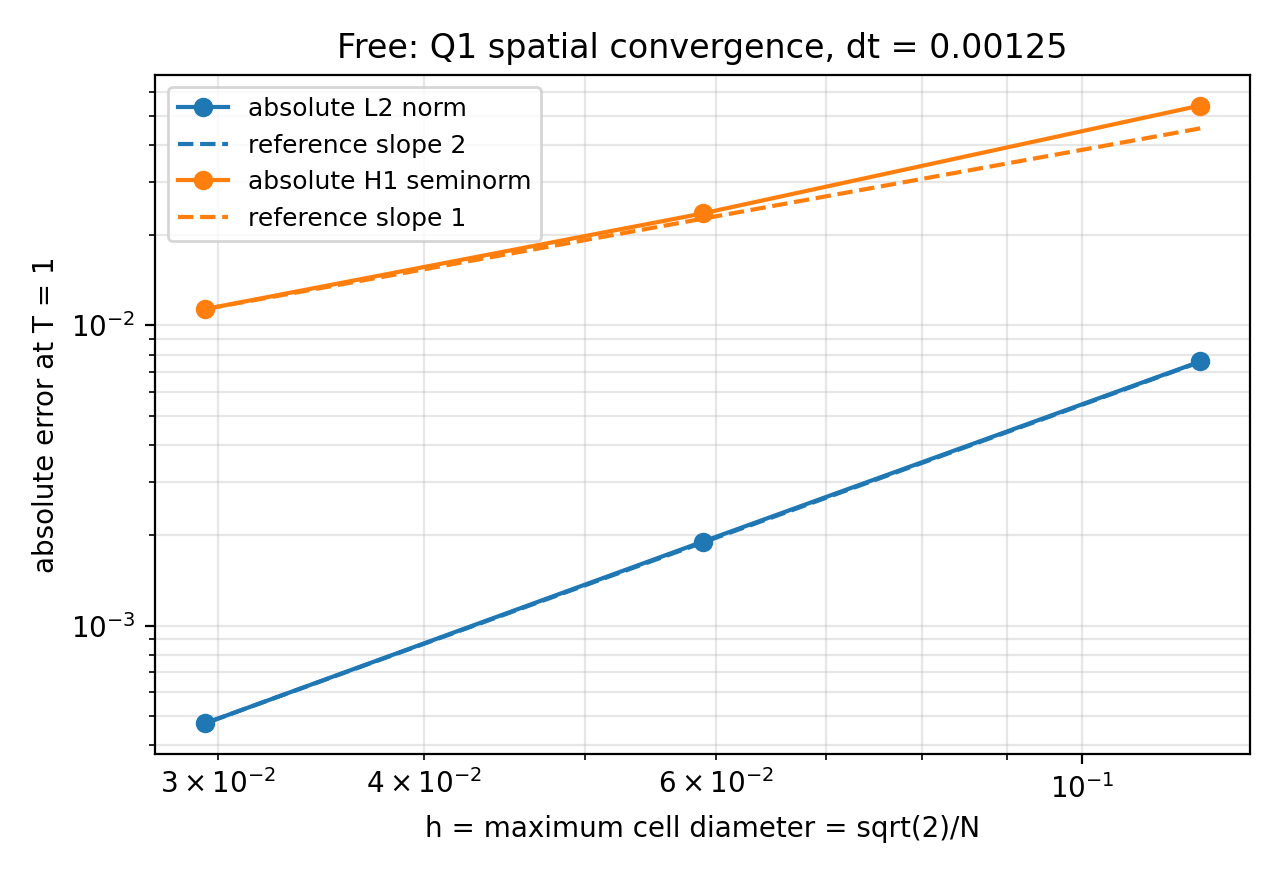
\includegraphics[width=0.82\textwidth]{../../assets/figures/free-convergence.png}
 \caption{Free solution: final absolute spatial errors versus maximum cell
 diameter on log--log axes. Dashed lines show Q1 reference slopes.}
\end{figure}
\begin{figure}[H]
 \centering
 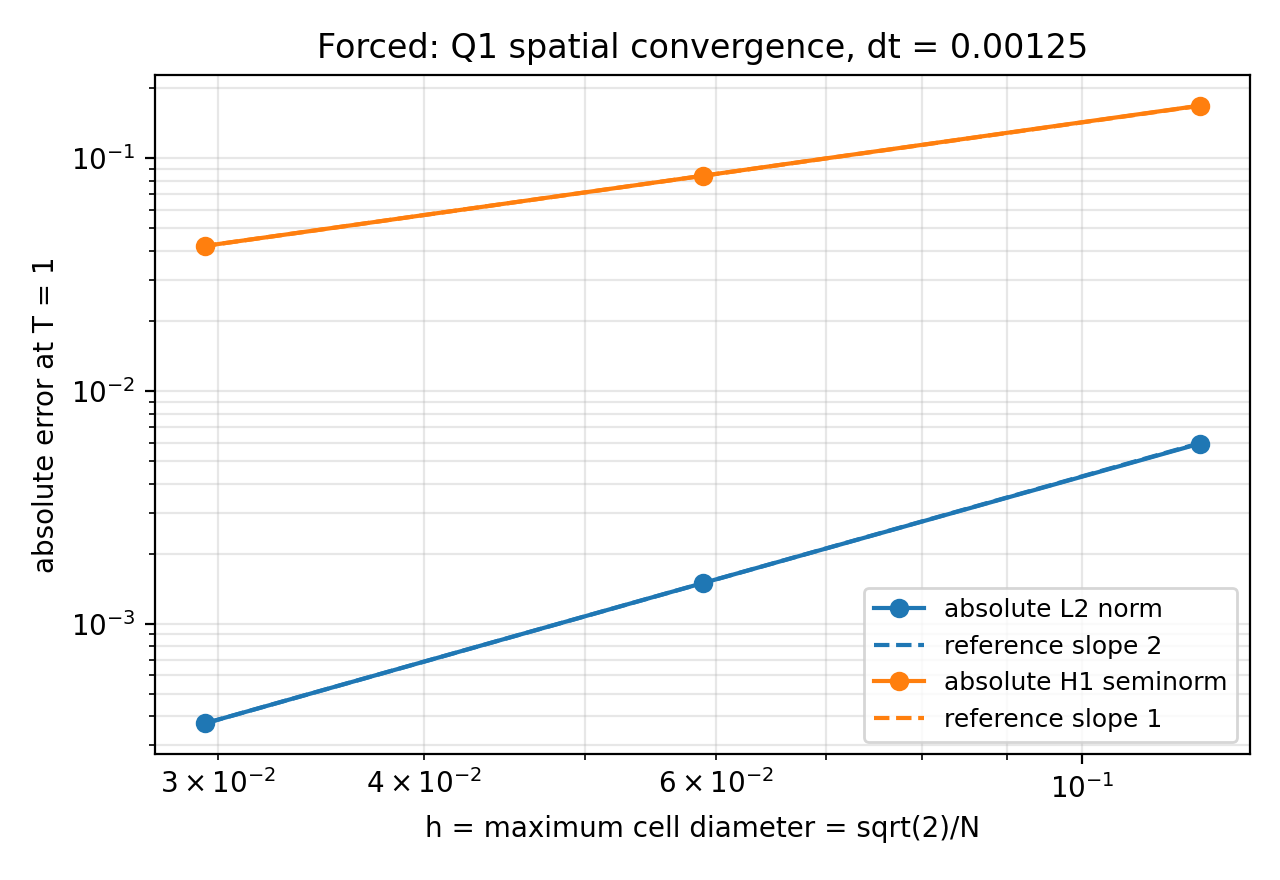
\includegraphics[width=0.82\textwidth]{../../assets/figures/forced-convergence.png}
 \caption{Forced solution: the same mesh-convergence experiment and norm
 definitions. These are not error-versus-time curves.}
\end{figure}

\section{Temporal Contamination Check}
For each mesh we halve \(\Delta t\) from 0.00125 to 0.000625, keeping
\(T=1\). The table reports
\(\left|e_{\Delta t/2}-e_{\Delta t}\right|/e_{\Delta t}\) for each final
error norm. The small changes support interpreting the mesh experiment as
predominantly spatial. They do not prove a rigorous bound on temporal error.
\begin{center}\small
\begin{tabular}{llll}
\toprule
case & N & $L^2$ change & $H^1$ change\\
\midrule
free & 12 & 5.435649e-04 & 1.914659e-04\\
free & 24 & 2.164670e-03 & 2.506564e-04\\
free & 48 & 8.719531e-03 & 2.703558e-04\\
forced & 12 & 1.124933e-04 & 1.386920e-06\\
forced & 24 & 4.504379e-04 & 1.406438e-06\\
forced & 48 & 1.804992e-03 & 1.408030e-06\\
\bottomrule
\end{tabular}\end{center}


The older validation suite uses \(\Delta t=0.0025\) for spatial refinement.
Its fixed-\(N=32\) tests at \(\Delta t=0.02,0.01,0.005\) mix spatial and temporal
errors. In particular, cancellation can make the total error increase as
the time step decreases. Those results are preserved in
\texttt{validation-summary.md} and are not presented as measured temporal
order. Second-order Newmark accuracy here is a theoretical property of the
scheme.

\section{Empirical Phase Check}
The phase formula in Chapter 3 can also be examined directly. We record the
displacement at the centre of the square, where the manufactured free solution
has its largest amplitude, and estimate the first numerical maximum by a
quadratic interpolation of the three samples around the discrete peak. The
exact period is \(2\pi/(\sqrt{2}\pi)=\sqrt{2}\). The experiment uses
\(N=192\), so the spatial contribution is small compared with the coarser
meshes used in the convergence study.

\begin{center}
\small
\begin{tabular}{rrrrr}
\toprule
$\Delta t$ & exact period & numerical peak & peak lag & phase lag (rad) \\
\midrule
0.02000 & 1.41421356 & 1.41513027 & 9.16702662e-04 & 4.07280262e-03 \\
0.01000 & 1.41421356 & 1.41443023 & 2.16668199e-04 & 9.62631444e-04 \\
0.00500 & 1.41421356 & 1.41425597 & 4.24077963e-05 & 1.88412875e-04 \\
\bottomrule
\end{tabular}
\end{center}


\begin{figure}[H]
 \centering
 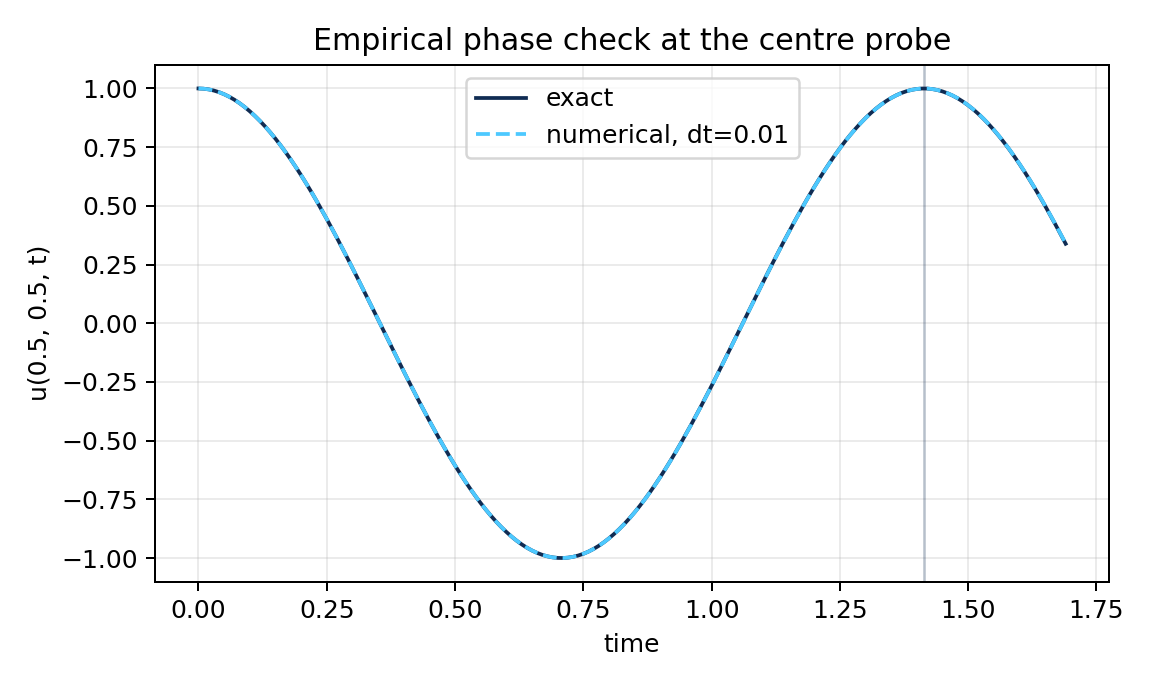
\includegraphics[width=0.78\textwidth]{../../assets/figures/dispersion-check.png}
 \caption{Centre-probe phase check for the free mode with \(\Delta t=0.01\).
 The numerical first peak is compared with the exact period; the vertical
 line marks the exact peak time.}
\end{figure}

The measured peak lag decreases from \(9.17\times10^{-4}\) to
\(4.24\times10^{-5}\) when the time step is reduced from \(0.02\) to \(0.005\),
consistent with the second-order phase error of average-acceleration Newmark.
The lag contains both spatial semi-discrete dispersion and temporal
dispersion, so this is an empirical consistency check rather than an isolated
measurement of temporal order.

\section{Error Evolution and Energy}
The following time curves use \(N=48\), \(Q_1\), \(\Delta t=0.00125\).
Each error sample is a spatial norm of the displacement error at that time.
Semilogarithmic vertical axes resolve small errors; the horizontal axis is
linear time.
\begin{figure}[H]
 \centering
 \begin{subfigure}{0.48\textwidth}
  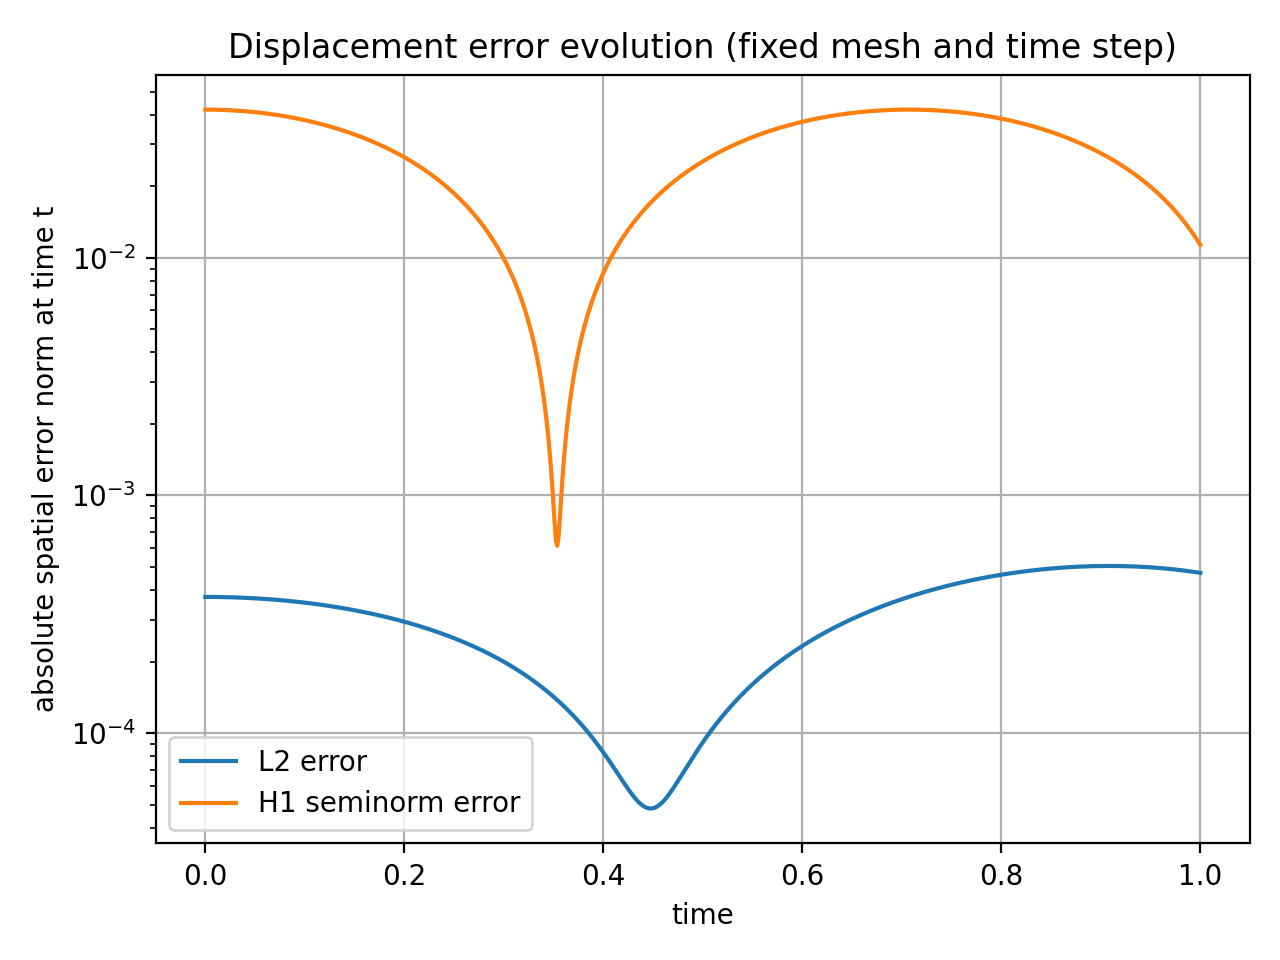
\includegraphics[width=\textwidth]{../../assets/figures/free-time-errors.png}
  \caption{Free: absolute errors versus time.}
 \end{subfigure}\hfill
 \begin{subfigure}{0.48\textwidth}
  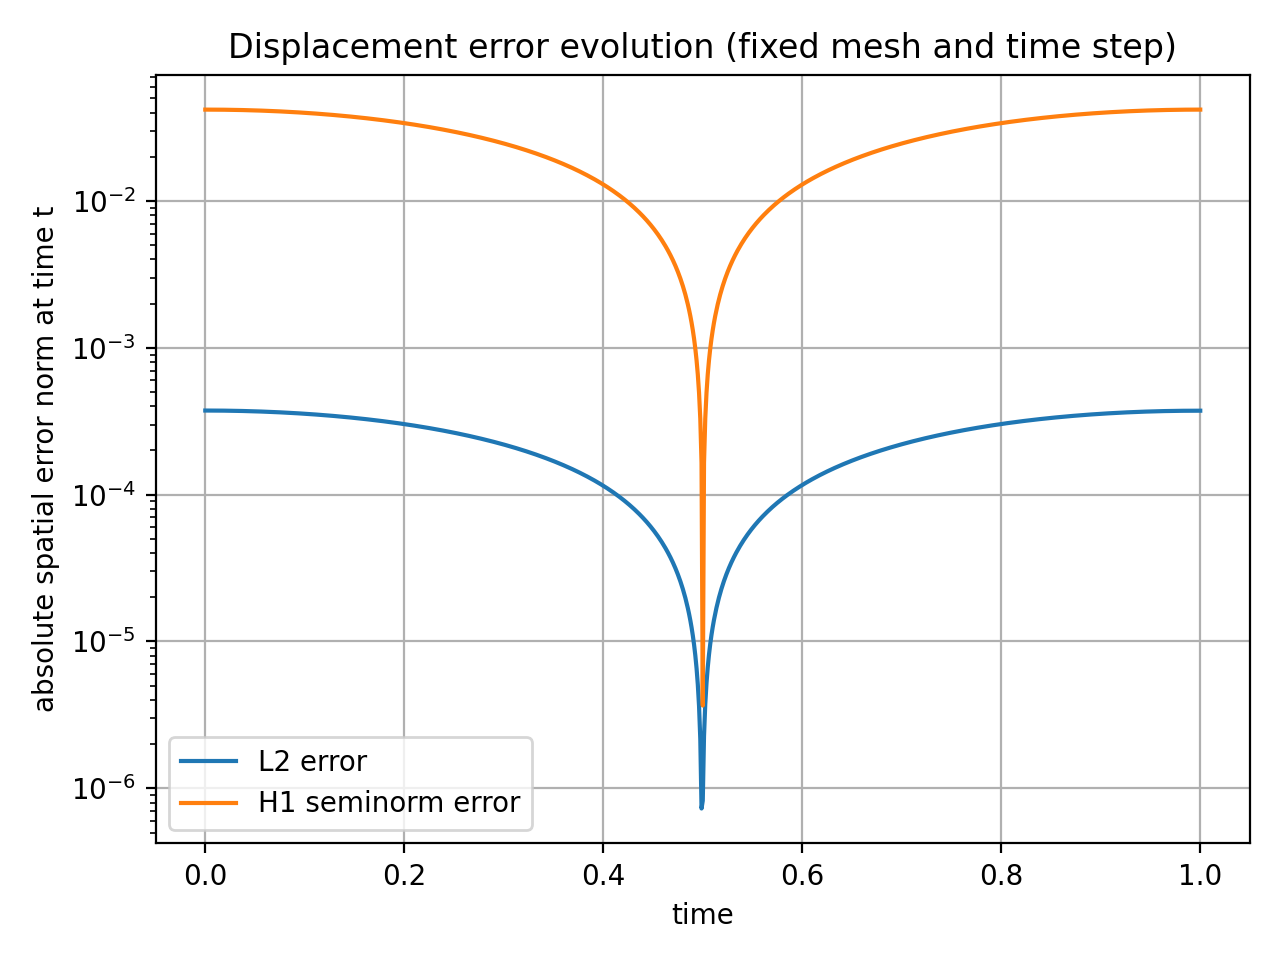
\includegraphics[width=\textwidth]{../../assets/figures/forced-time-errors.png}
  \caption{Forced: absolute errors versus time.}
 \end{subfigure}
 \caption{Time evolution on a fixed mesh, distinct from spatial convergence.}
\end{figure}

\begin{center}\small
\begin{tabular}{lllll}
\toprule
case & initial & final & minimum & max. rel. change\\
\midrule
free & 2.4647600926 & 2.4647600926 & 2.4647600926 & 5.225087e-15\\
forced & 2.4647600926 & 2.46476994554 & 1.23194254076 & 5.001775e-01\\
\bottomrule
\end{tabular}\end{center}

The last column is \(\max_n|E_h^n-E_h^0|/E_h^0\). It measures numerical drift
only for the free case. For the forced case it mainly measures physical
energy exchange. Energy is computed from the original \(M,K\); its initial
value differs slightly from the continuous \(\pi^2/4\) due to interpolation.

\begin{figure}[H]
 \centering
 \begin{subfigure}{0.48\textwidth}
  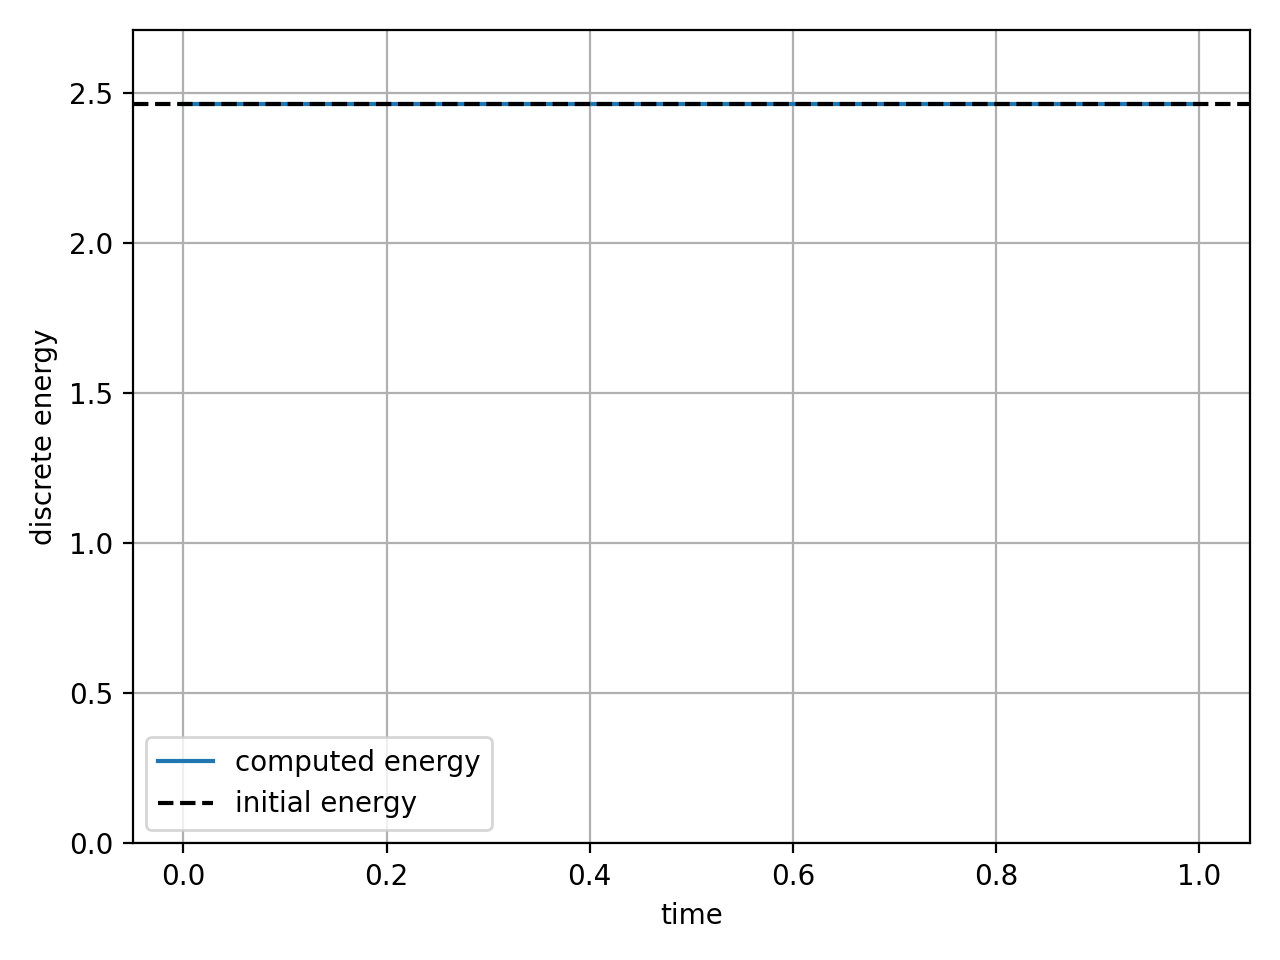
\includegraphics[width=\textwidth]{../../assets/figures/free-time-energy.png}
  \caption{Free mechanical energy.}
 \end{subfigure}\hfill
 \begin{subfigure}{0.48\textwidth}
  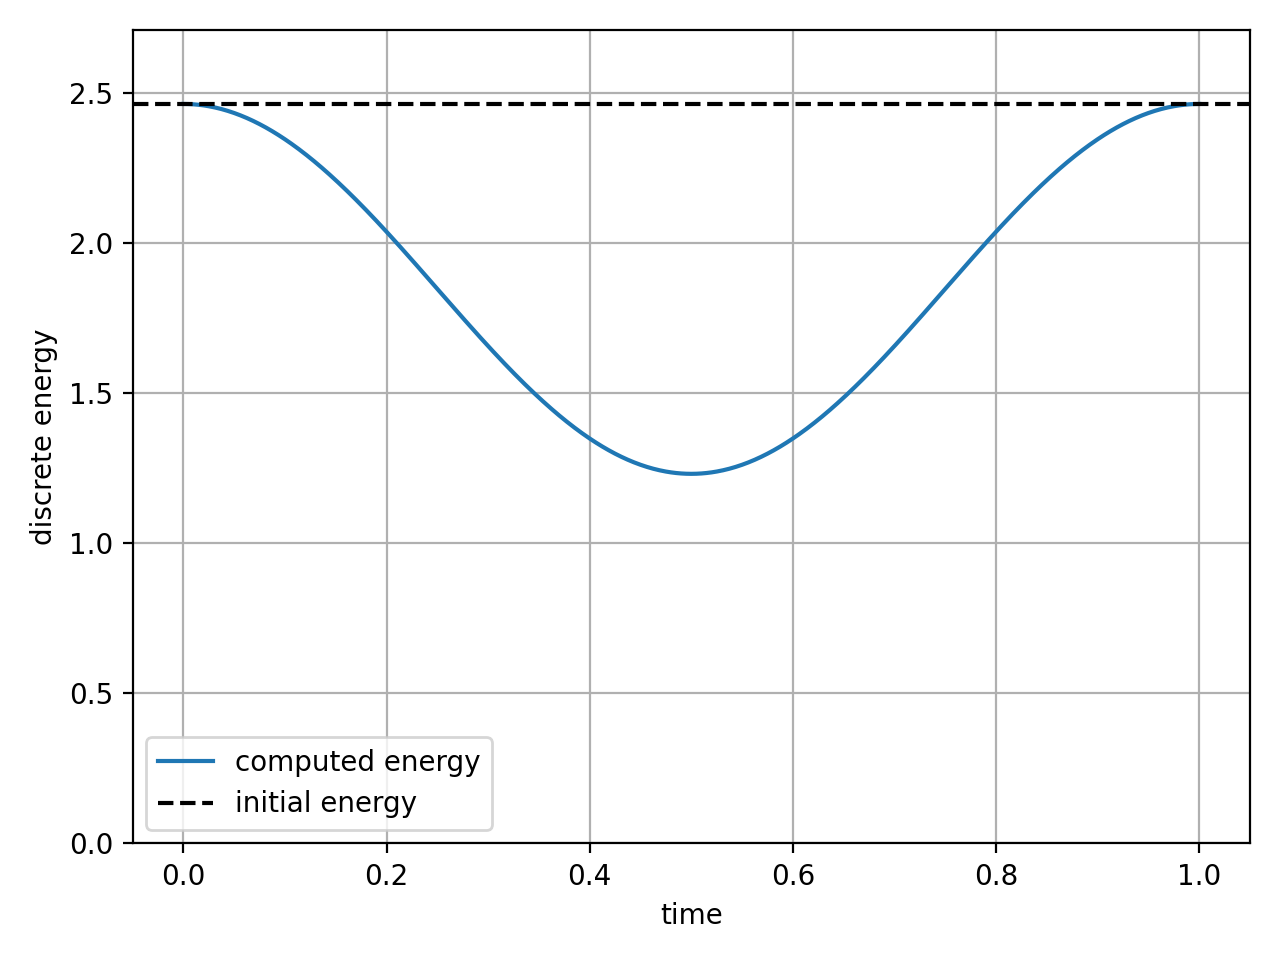
\includegraphics[width=\textwidth]{../../assets/figures/forced-time-energy.png}
  \caption{Forced mechanical energy.}
 \end{subfigure}
 \caption{Absolute energy with a zero baseline. Forcing removes and later
 returns energy; free energy is constant up to numerical error.}
\end{figure}
\begin{figure}[H]
 \centering
 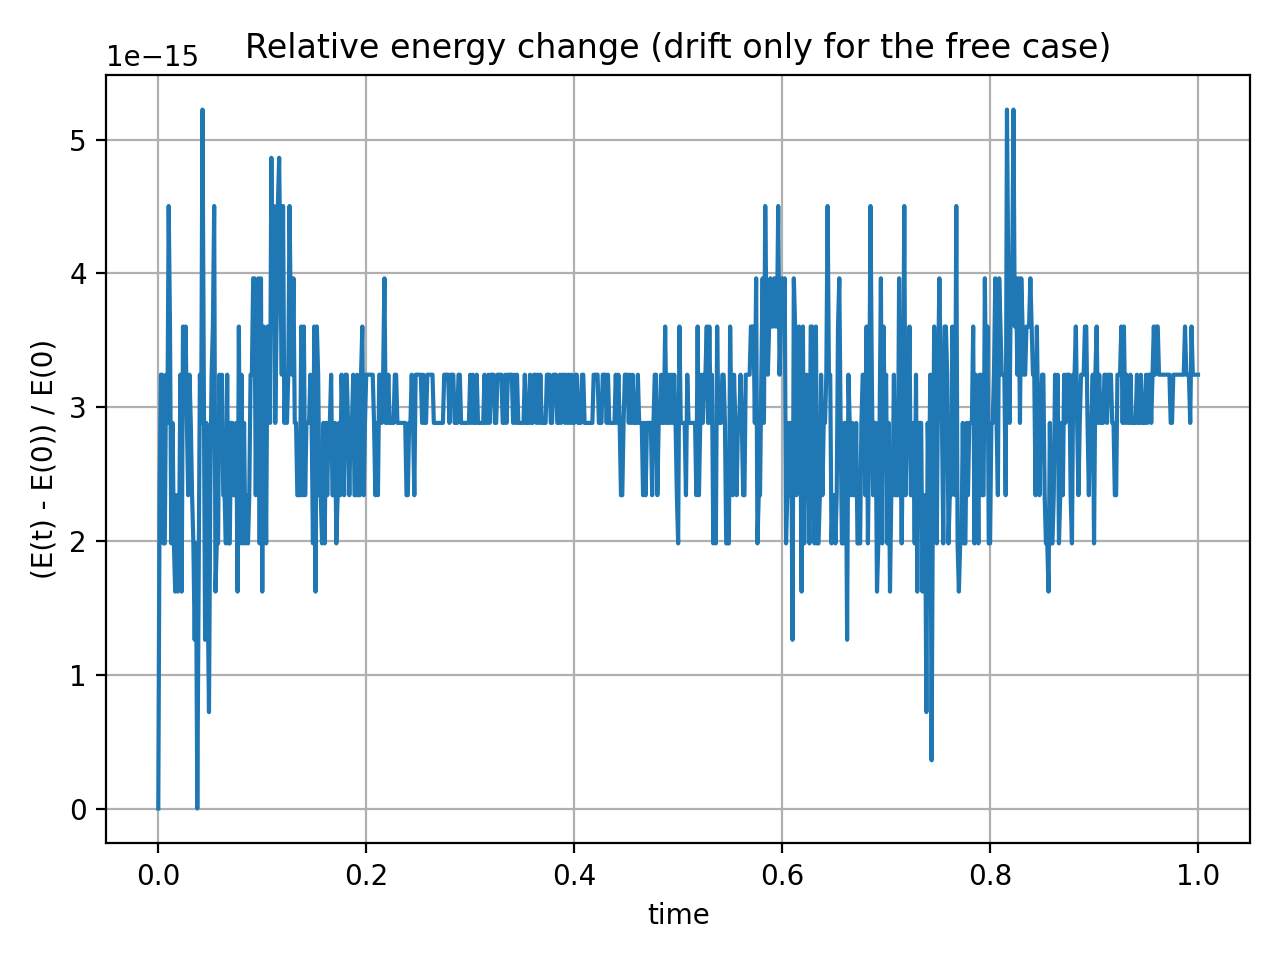
\includegraphics[width=0.78\textwidth]{../../assets/figures/free-time-energy_change.png}
 \caption{Free-case relative energy drift. The scale exposes small
 round-off/solver effects that are invisible on the absolute-energy plot.}
\end{figure}

\section{Solver Comparison}
All combinations solve the forced \(Q_1\), \(N=48\) problem (2401 stored
DoFs), \(T=0.1\), \(\Delta t=0.005\), on the same host in Release mode.
There are three repetitions per combination, all with the same stopping
tolerances and zero initial guesses. The initial mass solve is excluded
from this timing table. Mean iterations and maximum true residual are over
all 60 Newmark solves. Solve and preconditioner setup times are medians of
the totals for 20 time steps, in milliseconds. File output, assembly,
diagnostics and the independent residual recomputation are outside these timers.
\begin{center}\small
\begin{tabular}{lllllll}
\toprule
solver & prec. & converged & mean it. & max. residual & solve ms & setup ms\\
\midrule
cg & ssor & 3/3 & 6.00 & 2.615100e-12 & 29.87302 & 1.98151\\
cg & jacobi & 3/3 & 1.00 & 1.447179e-14 & 5.65763 & 0.06972\\
gmres & ssor & 3/3 & 6.00 & 2.605978e-12 & 44.73600 & 1.98325\\
gmres & jacobi & 3/3 & 1.00 & 1.425311e-14 & 6.06195 & 0.07157\\
\bottomrule
\end{tabular}\end{center}


All combinations agree in final errors and energy within relative tolerance
\(10^{-7}\) and absolute tolerance \(10^{-10}\). Sparse symmetry and
Rayleigh-quotient checks also pass; they supplement the SPD proof in Chapter 4.

Jacobi needs one iteration because the sine mode is an eigenvector of the
uniform-grid interior mass/stiffness operators and diagonal scaling preserves
it. SSOR need not preserve that eigenspace. This special result does not
predict general-load performance. CG+SSOR remains the baseline; timings are
machine-dependent and are not parallel scaling.


\newpage
\chapter{ParaView Visualization}

The solver writes ParaView files in \texttt{output/}. The main file to open is:
\begin{center}
  \texttt{output/wave\_solution.pvd}
\end{center}
The scalar field to visualize is \texttt{u}. A useful representation is
\texttt{Surface With Edges}; to see the membrane as a moving surface one can
apply the \texttt{Warp By Scalar} filter to the same field.

The three-dimensional surface in ParaView is only a visualization. The
mathematical problem is still two-dimensional in space: the height represents
the scalar value \(u(x,y,t)\).

At the initial time the displacement is positive in the center of the square
and zero on the boundary. During the simulation the membrane oscillates: the
central displacement decreases, crosses zero, changes sign, and later returns
towards the initial shape. This is the behavior expected from the selected
manufactured solution, which has a cosine dependence in time.

\begin{figure}[H]
  \centering
  \begin{subfigure}{0.48\textwidth}
    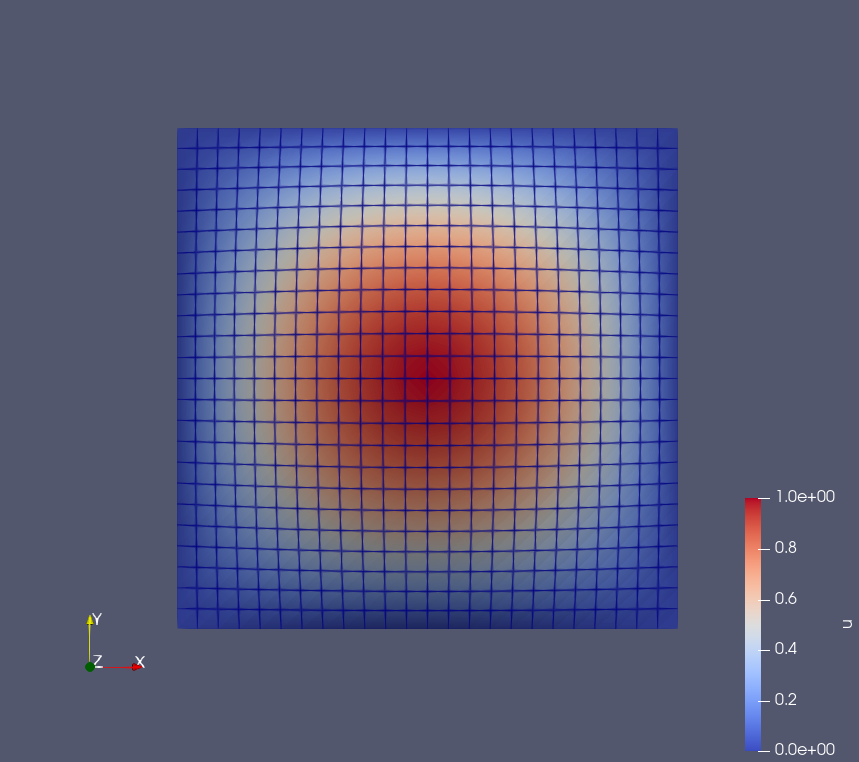
\includegraphics[width=\textwidth]{../../assets/paraview-screenshots/solution_u_t0_2d.png}
    \caption{Scalar field on the 2D mesh.}
  \end{subfigure}
  \hfill
  \begin{subfigure}{0.48\textwidth}
    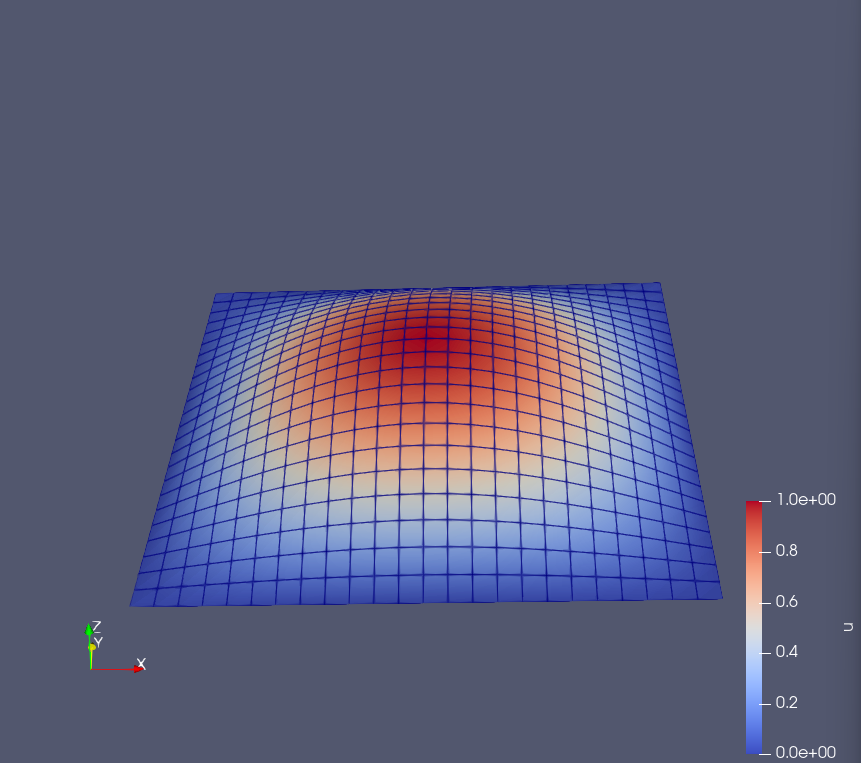
\includegraphics[width=\textwidth]{../../assets/paraview-screenshots/solution_u_t0_warped.png}
    \caption{Warped view of the same scalar field.}
  \end{subfigure}
  \caption{Initial displacement visualized in ParaView.}
\end{figure}

\begin{figure}[H]
  \centering
  \begin{subfigure}{0.48\textwidth}
    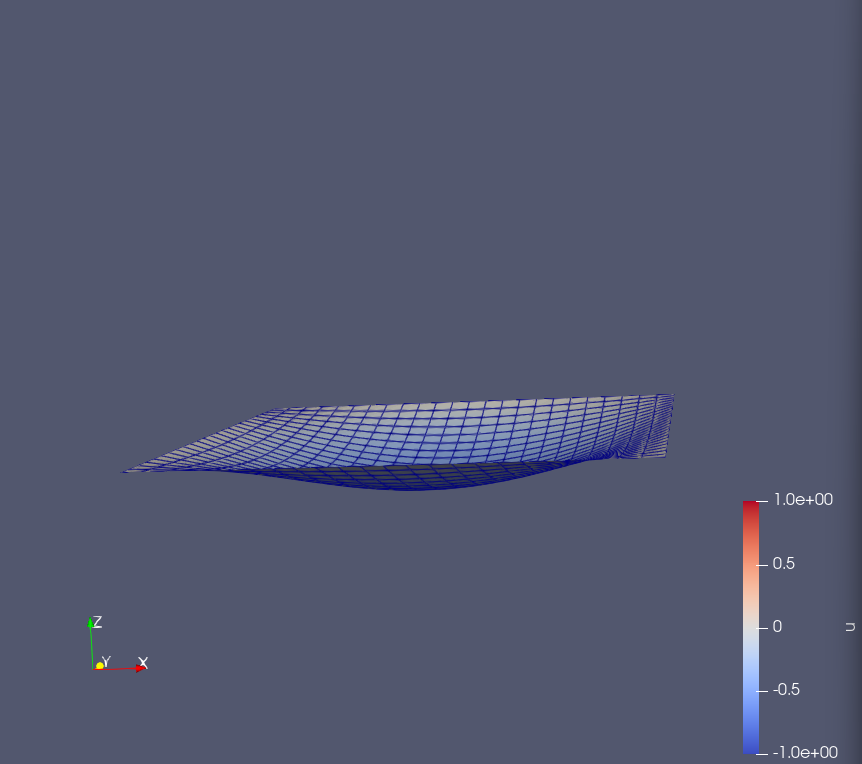
\includegraphics[width=\textwidth]{../../assets/paraview-screenshots/solution_u_t10_warped.png}
    \caption{Intermediate warped view.}
  \end{subfigure}
  \hfill
  \begin{subfigure}{0.48\textwidth}
    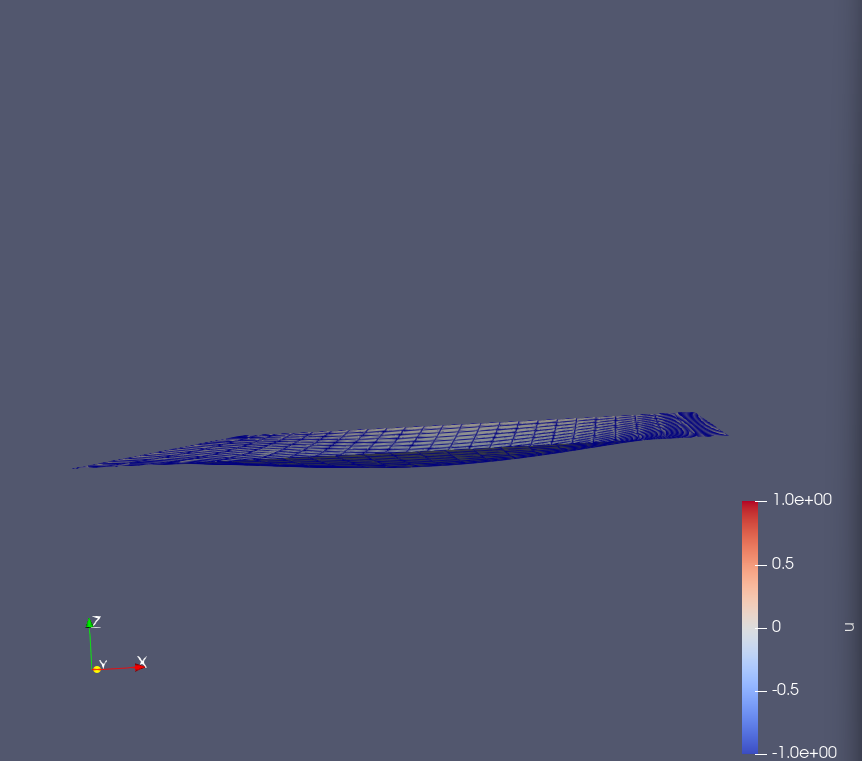
\includegraphics[width=\textwidth]{../../assets/paraview-screenshots/solution_u_t20_warped.png}
    \caption{Later warped view.}
  \end{subfigure}
  \caption{Time evolution of the membrane displacement in ParaView.}
\end{figure}

These are the group's existing qualitative screenshots. Their filenames
\texttt{t10} and \texttt{t20} do not establish physical times: no timestamp or
saved ParaView state accompanies them. They are retained as illustrations,
not used for error measurements or claimed to belong to the new convergence
study. For reproducible time labels, read the PVD time value in ParaView.


\newpage
\chapter{Conclusions and HPC Scope}
\small
\sloppy

\section{Conclusions}
This project combines a conforming bilinear \(Q_1\) finite-element
discretization on a structured square mesh with Newmark average acceleration
for the wave equation. The implementation assembles the spatial operators once,
solves one constant effective system at each time step, and evaluates the
solution through errors, energy diagnostics, VTK output and a centre-point phase
probe.

The manufactured-solution experiments give approximately second-order
convergence in the displacement \(L^2\) norm and first-order convergence in the
\(H^1\) seminorm. The free-case energy drift is at round-off level for the
tested run, whereas the forced-case energy changes because the external load
does work. The effective Newmark matrix is symmetric positive definite after
homogeneous Dirichlet elimination, which justifies conjugate gradients; sparse
symmetry and Rayleigh-quotient checks were used as numerical diagnostics in
addition to this mathematical argument. The empirical centre-probe experiment
also shows the expected phase sensitivity to the time step.

\section{MPI Implementation and Measurements}
The repository contains two executable paths. \texttt{wave\_fem} is the
serial reference used for the controlled verification studies. The completed
\texttt{wave\_fem\_mpi} implementation distributes the structured mesh and
degrees of freedom with the distributed deal.II triangulation, uses
distributed Trilinos matrices and vectors, computes global diagnostics through
MPI reductions, and writes distributed VTK snapshots.

We compared the original serial executable with the MPI executable on the same
problem, \(N=192\), \(T=0.1\), and \(\Delta t=0.0025\), using the same
initial/final output policy and diagnostics at every time step. The serial run
took 14.533 s, while MPI took 13.823 s with one rank, 11.529 s with two ranks
and 7.339 s with four ranks; the final numerical errors agree. MPI-1 is only a
slight improvement over serial, while MPI-4 gives a speedup of 1.98 and an
efficiency of 49.5% relative to the serial baseline. The comparison still
reflects different sparse backends, so it is an end-to-end implementation
comparison rather than a backend-independent kernel benchmark.

Within MPI, the time loop takes 12.322 s, 10.183 s and 6.361 s for one, two and
four ranks. The time-loop component decreases from 12.322 s on one rank to
6.361 s on four ranks, but the efficiency remains below ideal because each
rank participates in synchronisation and distributed sparse solves. The
communications are required to exchange interface data and form global
diagnostics; their cost is only partly amortised by the available local work.

The timer starts before mesh setup and stops after diagnostics and VTK output.
Each reported phase is the maximum elapsed time over the MPI ranks, so the
measurement represents the wall-clock time of the parallel job rather than an
average rank time.

\begin{center}
\small
\begin{tabular}{lrrrrrrr}
\toprule
Implementation & Ranks & DoFs & Cells & Setup (s) & Time loop (s) & Post-process (s) & Total (s) \\
\midrule
serial & 1 & 37249 & 36864 & -- & -- & -- & 14.533 \\
MPI & 1 & 37249 & 36864 & 1.177 & 12.322 & 0.324 & 13.823 \\
MPI & 2 & 37249 & 36864 & 1.148 & 10.183 & 0.198 & 11.529 \\
MPI & 4 & 37249 & 36864 & 0.865 & 6.361 & 0.158 & 7.339 \\
\bottomrule
\end{tabular}
\end{center}


\begin{figure}[H]
 \centering
 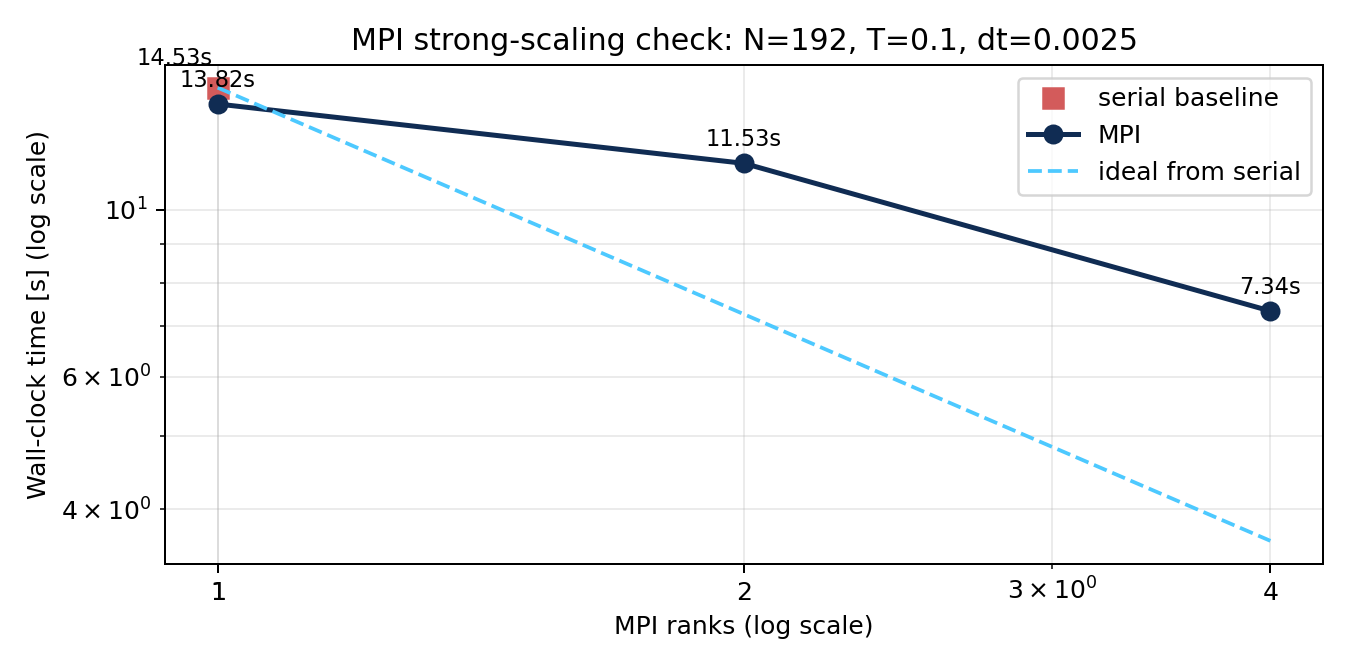
\includegraphics[width=0.78\textwidth]{../../assets/figures/mpi-scaling-loglog.png}
 \caption{End-to-end MPI time versus process count on log--log axes. The
 dashed line is ideal inverse-rank scaling from the one-rank measurement.}
\end{figure}

This is the scalability result obtained in our HPC study, not evidence that the
MPI implementation is missing. It characterises the small-problem regime in
which fixed MPI costs dominate. Increasing the problem size or changing the
machine would let us investigate the complementary strong-scaling regime, but
that is a different experimental regime rather than an unfinished part of the
implementation.

The serial problem-size study in \texttt{run\_scalability\_study.sh} is kept
separate from MPI scaling. Increasing \(N\) there measures the growth of the
serial computational problem; it is not labelled strong or weak scaling.

The validation is intentionally bounded to smooth manufactured standing-wave
data, the unit square and homogeneous Dirichlet conditions. It therefore does
not claim accuracy for nonsmooth data, arbitrary geometries or long-time
propagation.

\small
\begin{thebibliography}{9}
\bibitem{arnold}
D. N. Arnold, D. Boffi, R. S. Falk,
\emph{Approximation by quadrilateral finite elements}.
\url{https://arxiv.org/abs/math/0005036}.
\bibitem{dealii}
deal.II 9.5, \emph{FE\_Q documentation}.
\url{https://dealii.org/9.5.0/doxygen/deal.II/classFE__Q.html}.
Solver and boundary APIs were also checked against the installed 9.5.1 headers.
\bibitem{newmark}
N. M. Newmark, ``A method of computation for structural dynamics,''
\emph{Journal of the Engineering Mechanics Division}, ASCE, 85(EM3),
67--94, 1959.
\bibitem{course}
M. Bucelli, \emph{NMPDE project repository template}.
\url{https://github.com/michelebucelli/nmpde-projects}.
\end{thebibliography}


\end{document}
